\begin{figure}[h!]
\begin{center}
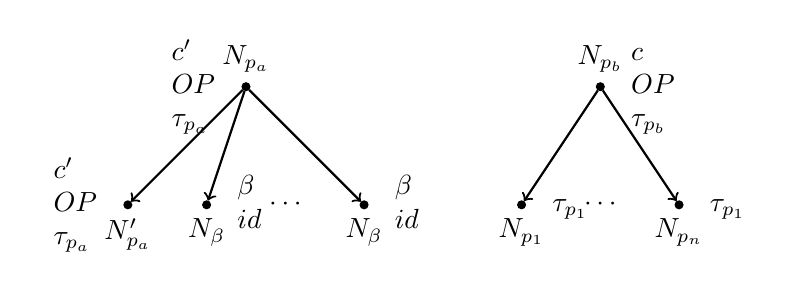
\begin{tikzpicture}[yscale=-1,
place/.style={circle,draw=black, fill=black, inner sep=0pt, 
              minimum size=1mm}]

  \node[place] (1st) at (1.5, 0) [label=above: $N_{p_a}$,
                                  label=left: 
     \begin{tabular}{l}
        $c'$\\
        $OP$\\
        $\tau_{p_a}$\\  
     \end{tabular}
] {};
  \node[place] (2nd) at (0, 1.5) [label=below: $N'_{p_a}$,
                                  label=left:
     \begin{tabular}{l}
        $c'$\\
        $OP$\\
        $\tau_{p_a}$\\  
     \end{tabular}
]{};
  \node[place] (3rd) at (1, 1.5) [label=below: $N_{\beta}$, 
    label=right: 
             \begin{tabular}{l}
            $\beta$\\
            $id$\\
             \end{tabular}
	] {}; 
  \node[place] (4th) at (3, 1.5) [label=below: $N_{\beta}$,
    label=right: 
             \begin{tabular}{l}
            $\beta$\\
            $id$\\
             \end{tabular}
             ] {}; 

  \node (dots) at (2,1.5) {$\cdots$};
	
  \draw[->, thick] (1st) -- (2nd);
  \draw[->, thick] (1st) -- (3rd);
  \draw[->, thick] (1st) -- (4th);

\begin{scope}[xshift=5cm]
  \node[place] (1st) at (1, 0) [label=above: $N_{p_b}$,
                                label=right: 
     \begin{tabular}{l}
        $c$\\
        $OP$\\
        $\tau_{p_b}$\\
     \end{tabular}
] {};
  \node[place] (2nd) at (0, 1.5) [label=below: $N_{p_1}$, 
    label=right: 
             \begin{tabular}{l}
            $\tau_{p_1}$\\
             \end{tabular}
             ] {};
  \node[place] (3rd) at (2, 1.5) [label=below: $N_{p_n}$, 
  label=right: 
             \begin{tabular}{l}
            $\tau_{p_1}$\\
             \end{tabular}
             ] {}; 

  \node (dots) at (1,1.5) {$\cdots$};
	
  \draw[->, thick] (1st) -- (2nd);
  \draw[->, thick] (1st) -- (3rd);
\end{scope}

);
\end{tikzpicture}
\end{center}
\caption{Comparison between atomic and complex predicates}
\label{fig:SimAC}
\end{figure}